\chapter{Project Specification}
Summary of the project outline.

\section{Functional Requirements}
some text here

\section{Non-Functional Requirements}
some text here

\chapter{Project Management}
Discussion on how the project was managed. What things impacted the success of the project. How does the continually revised versions of the project plan compare to the initial draft developed at the start of the project. Did everything run according the schedule. Did elements such as exams \& coursework have any impact. 

\chapter{Another Appendix}

This appendix makes use of the \emph{rotating} package to rotate both figures and tables ninety degrees allowing for large datasets and illustrations to be represented.

\begin{sidewaystable}
\begin{center}
   \begin{tabular}{llllllllll} 
   \toprule
   \textbf{Heading 1} & \textbf{Heading 2}  & \textbf{Heading 3}  & \textbf{Heading 4}  & \textbf{Heading 5}  & \textbf{Heading 6}  & \textbf{Heading 7}  & \textbf{Heading 8}  & \textbf{Heading 9}  & \textbf{Heading 10}  \cr
   \midrule
   aaa & bbbb & cccc & dddd & eeee & ffff & gggg & hhhh & iiii & jjjj \cr 
   aaa & bbbb & cccc & dddd & eeee & ffff & gggg & hhhh & iiii & jjjj \cr 
   aaa & bbbb & cccc & dddd & eeee & ffff & gggg & hhhh & iiii & jjjj \cr 
   aaa & bbbb & cccc & dddd & eeee & ffff & gggg & hhhh & iiii & jjjj \cr 
   aaa & bbbb & cccc & dddd & eeee & ffff & gggg & hhhh & iiii & jjjj \cr 
   aaa & bbbb & cccc & dddd & eeee & ffff & gggg & hhhh & iiii & jjjj \cr 
   \bottomrule
   \end{tabular}
\caption[A Short Caption for the table]{
	A much longer caption that will not be listed in the list of tables page.
}
\label{tab:sidewaysTable}
\end{center}
\end{sidewaystable}

\begin{sidewaysfigure}
\centerline{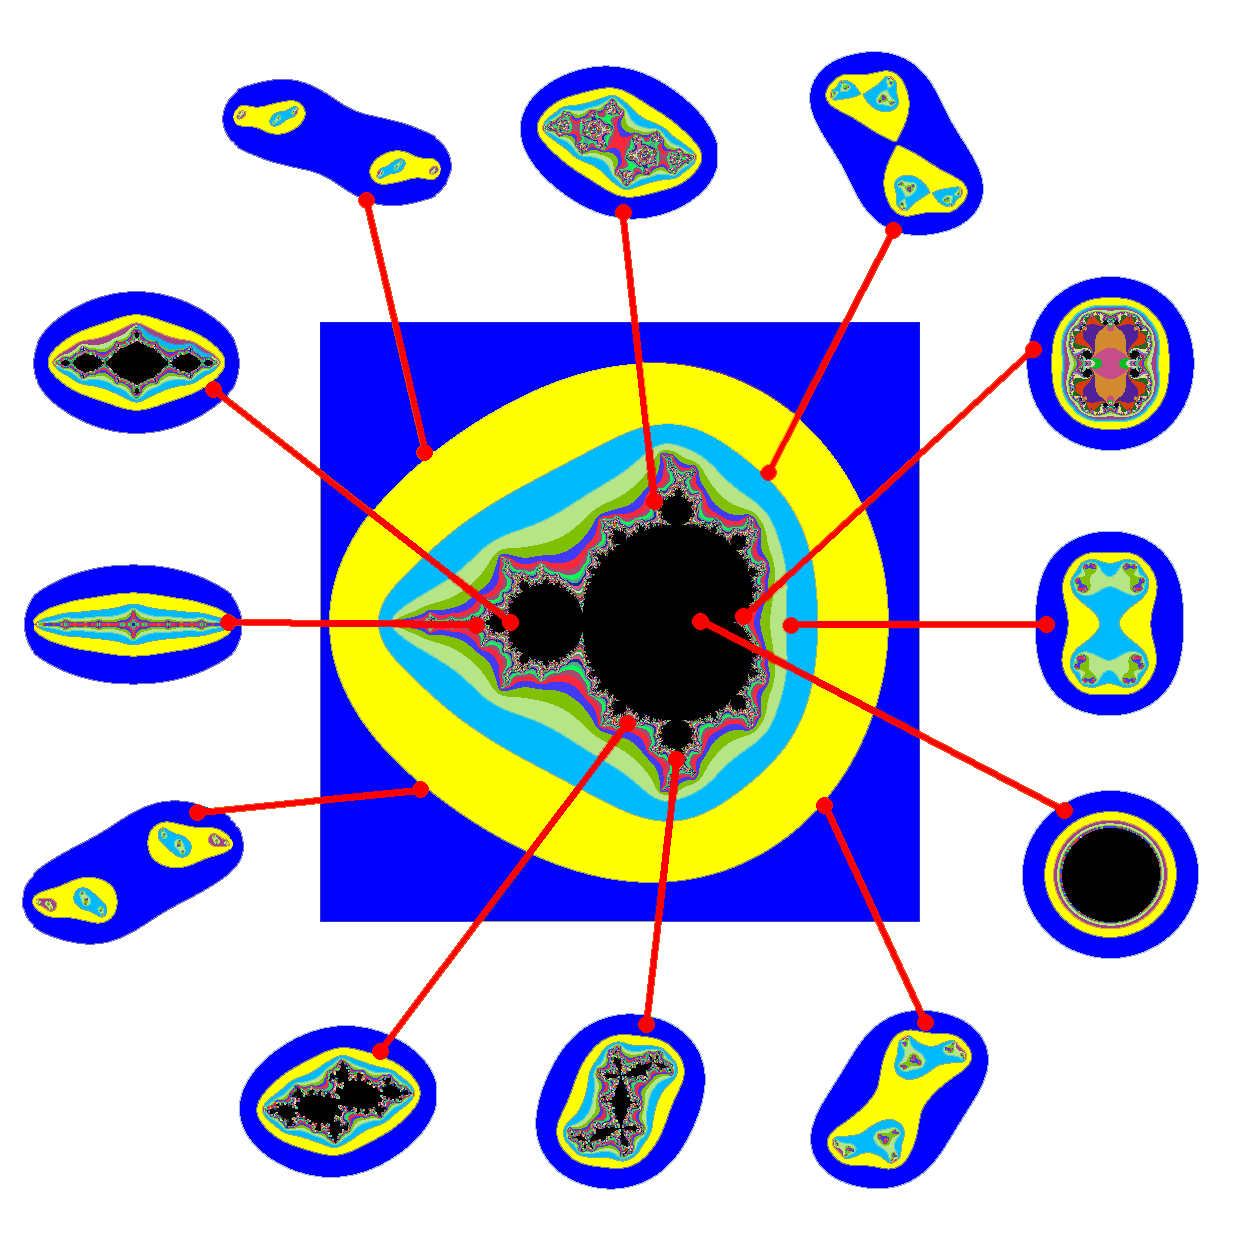
\includegraphics[width=7in]{appendix/images/samplepng}}
\caption[A Sideways Figure]{
	A much longer caption that will not be listed in the list of figures page.
}
\label{fig:sidewaysFigure}
\end{sidewaysfigure}

\chapter{Presentation Slides}

The slides from the formal presentation should be provided here in not more than two pages. 

\chapter{Project Log}

The following is a weekly summary of the work carried during the development of this body of work. It covers tasks that were completed, tutorials that were worked through, articles that were read and reviews of discussions / meetings held with the project supervisor and other third parties. 

\section*{Week Beginning: Monday 27/09/2010}

First week working on the project. Had a meeting with supervisor and discussed some of the issues related to the project. The first deliverable is due for the end of next week (project outline \& ethics form). 

\begin{itemize}
  \item Downloaded and Installed \LaTeX \space (MikTeX full install), Ghostscript, Ghostview \& Winshell. 
  \item Started to get to grips with the \LaTeX \space system by making simple modifications to the template and editing the project log.
  \item Developed a Mind Map to clarify understanding of project elements.
  \item Prepared an initial draft of project plan in the form of a Gantt chart. 
  \item Prepared and revised 1 page draft of project summary \& filled in ethics form. 
\end{itemize}



